\documentclass[tikz,border=3pt]{standalone}
% Shared preamble for every TikZ figure in the report.
% Colours are Okabe-Ito, with roles fixed across all nine figures.
\usepackage[T1]{fontenc}
\usepackage{lmodern}
\usepackage{amsmath,amssymb}
\usetikzlibrary{arrows.meta,positioning,calc,fit,backgrounds,shapes.geometric,shapes.misc,decorations.pathreplacing,patterns}

\definecolor{cGraph}{HTML}{0072B2}
\definecolor{cSem}{HTML}{E69F00}
\definecolor{cFuse}{HTML}{009E73}
\definecolor{cLoop}{HTML}{D55E00}
\definecolor{cOracle}{HTML}{CC79A7}
\definecolor{cNeutral}{HTML}{999999}
\definecolor{cInk}{HTML}{222222}

\tikzset{
  every picture/.style={line width=0.5pt},
  box/.style={draw=cNeutral!90!black, fill=cNeutral!8, rounded corners=1.6pt,
              align=center, inner sep=3.2pt, font=\small, text=cInk},
  gbox/.style={box, draw=cGraph, fill=cGraph!7},
  sbox/.style={box, draw=cSem!80!black, fill=cSem!12},
  fbox/.style={box, draw=cFuse, fill=cFuse!8},
  lbox/.style={box, draw=cLoop, fill=cLoop!8},
  ann/.style={font=\scriptsize, text=cInk, align=center, inner sep=1.5pt},
  flow/.style={-{Stealth[length=4pt,width=3.2pt]}, draw=cNeutral!85!black},
  gflow/.style={flow, draw=cGraph},
  sflow/.style={flow, draw=cSem!85!black},
}

% Figure labels are short; never hyphenate them.
\hyphenpenalty=10000
\exhyphenpenalty=10000

\tikzset{
  pstep/.style={draw=cInk!70, fill=white, rounded corners=1.6pt, align=center,
               inner sep=3pt, font=\small, text=cInk, text width=3.1cm, minimum height=8mm},
  num/.style={circle, fill=cInk, text=white, font=\tiny\bfseries, inner sep=1.4pt,
              minimum size=3.6mm},
  mech/.style={font=\scriptsize, text=cInk!75, align=center, inner sep=1pt},
  leg/.style={font=\scriptsize, text=cInk!85, anchor=west, inner sep=1pt},
}
\newcommand{\tr}[1]{\\[2.5pt]{\itshape\color{cLoop}#1}}
\begin{document}
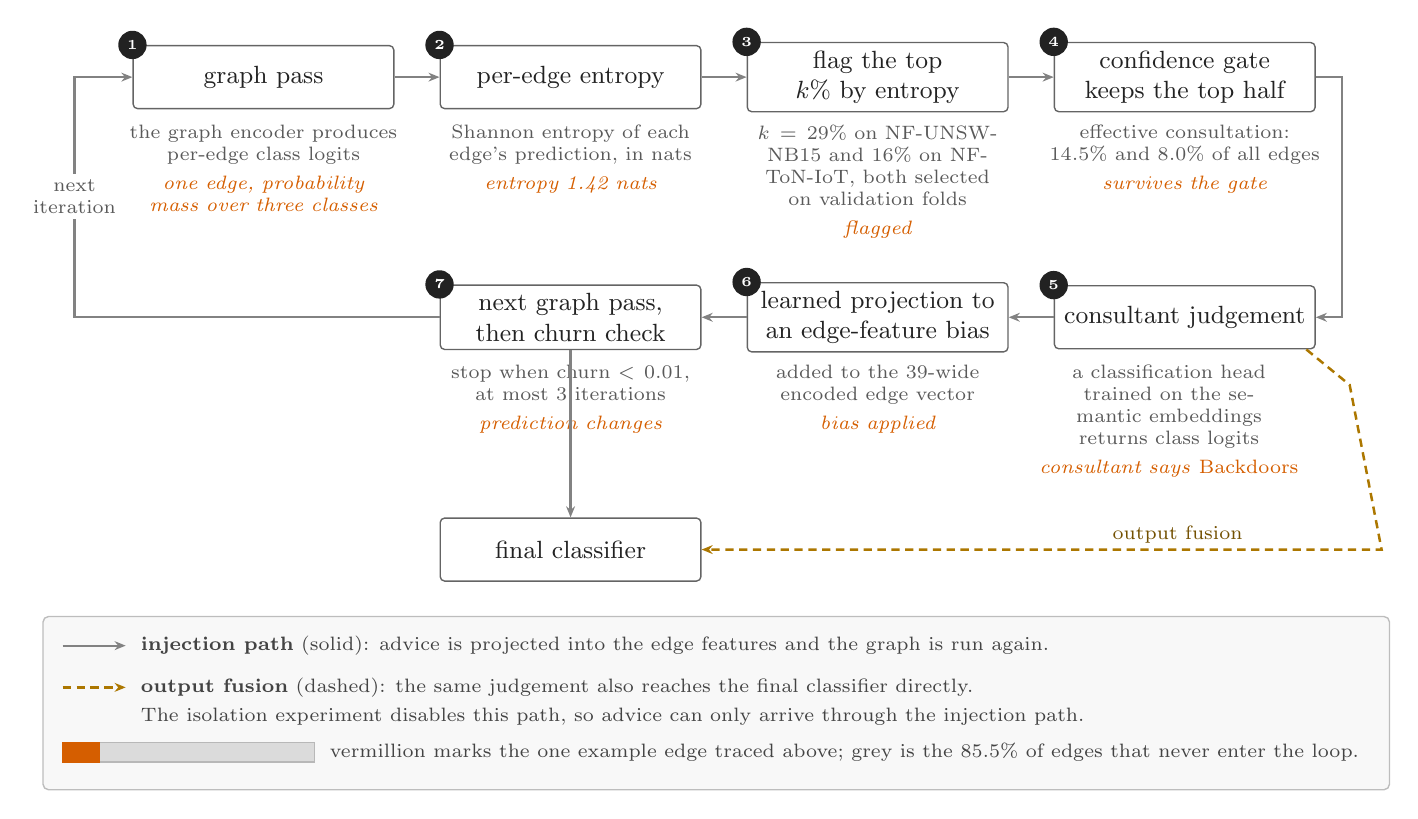
\begin{tikzpicture}[x=1cm,y=1cm]

\def\rA{2.30}
\def\rB{-0.75}

% ---------------------------------------------------------------- the seven steps
\node[pstep] (s1) at (1.85,\rA) {graph pass};
\node[pstep] (s2) at (5.75,\rA) {per-edge entropy};
\node[pstep] (s3) at (9.65,\rA) {flag the top $k\%$ by entropy};
\node[pstep] (s4) at (13.55,\rA) {confidence gate keeps the top half};
\node[pstep] (s5) at (13.55,\rB) {consultant judgement};
\node[pstep] (s6) at (9.65,\rB) {learned projection to an edge-feature bias};
\node[pstep] (s7) at (5.75,\rB) {next graph pass, then churn check};

\foreach \n/\s in {1/s1,2/s2,3/s3,4/s4,5/s5,6/s6,7/s7}
  \node[num] at (\s.north west) {\n};

% ---------------------------------------------------------------- the injection path
\draw[flow, line width=0.8pt] (s1) -- (s2);
\draw[flow, line width=0.8pt] (s2) -- (s3);
\draw[flow, line width=0.8pt] (s3) -- (s4);
\draw[flow, line width=0.8pt] (s4.east) -- (15.55,\rA) -- (15.55,\rB) -- (s5.east);
\draw[flow, line width=0.8pt] (s5) -- (s6);
\draw[flow, line width=0.8pt] (s6) -- (s7);
\draw[flow, line width=0.8pt] (s7.west) -- (-0.55,\rB) -- (-0.55,\rA) -- (s1.west);
\node[mech, fill=white, inner sep=2pt] at (-0.55,0.78) {next\\ iteration};

% ---------------------------------------------------------------- annotations and trace
\node[mech, anchor=north, text width=3.5cm] at (1.85,\rA-0.56)
      {the graph encoder produces per-edge class logits\tr{one edge, probability mass over three classes}};
\node[mech, anchor=north, text width=3.5cm] at (5.75,\rA-0.56)
      {Shannon entropy of each edge's prediction, in nats\tr{entropy 1.42 nats}};
\node[mech, anchor=north, text width=3.7cm] at (9.65,\rA-0.56)
      {$k=29\%$ on NF-UNSW-NB15 and $16\%$ on NF-ToN-IoT, both selected on validation folds\tr{flagged}};
\node[mech, anchor=north, text width=3.7cm] at (13.55,\rA-0.56)
      {effective consultation: $14.5\%$ and $8.0\%$ of all edges\tr{survives the gate}};

\node[mech, anchor=north, text width=3.3cm] at (13.35,\rB-0.56)
      {a classification head trained on the semantic embeddings returns class logits\tr{consultant says \emph{Backdoors}}};
\node[mech, anchor=north, text width=3.5cm] at (9.65,\rB-0.56)
      {added to the 39-wide encoded edge vector\tr{bias applied}};
\node[mech, anchor=north, text width=3.5cm] at (5.75,\rB-0.56)
      {stop when churn $<0.01$, at most 3 iterations\tr{prediction changes}};

% ---------------------------------------------------------------- the second path
\node[pstep] (fin) at (5.75,-3.70) {final classifier};
\draw[flow, line width=0.8pt] (s7.south) -- (fin.north);
\draw[flow, dashed, dash pattern=on 3pt off 2pt, draw=cSem!75!black, line width=0.9pt]
      ($(s5.south east)+(-0.12,0)$) -- ++(0.55,-0.45) -- (16.05,-3.70) --
      node[mech, above, text=cSem!50!black, fill=white, inner sep=2pt, pos=0.30]
      {output fusion} (fin.east);

% ---------------------------------------------------------------- legend
\draw[draw=cInk!30, fill=cInk!3, rounded corners=2pt] (-0.95,-4.55) rectangle (16.15,-6.75);

\draw[flow, line width=0.8pt] (-0.70,-4.92) -- (0.10,-4.92);
\node[leg] at (0.25,-4.92)
     {\textbf{injection path} (solid): advice is projected into the edge features and the graph is run again.};

\draw[flow, dashed, dash pattern=on 3pt off 2pt, draw=cSem!75!black, line width=0.9pt]
     (-0.70,-5.45) -- (0.10,-5.45);
\node[leg] at (0.25,-5.45)
     {\textbf{output fusion} (dashed): the same judgement also reaches the final classifier directly.};
\node[leg] at (0.25,-5.82)
     {The isolation experiment disables this path, so advice can only arrive through the injection path.};

\draw[fill=cNeutral!35, draw=cNeutral!70] (-0.70,-6.40) rectangle (2.50,-6.15);
\draw[fill=cLoop, draw=cLoop] (-0.70,-6.40) rectangle (-0.24,-6.15);
\node[leg] at (2.65,-6.27)
     {vermillion marks the one example edge traced above; grey is the $85.5\%$ of edges that never enter the loop.};

\end{tikzpicture}
\end{document}
